%% FELthesis: LaTeX class for bachelor, master, and phd thesis in CTU FEL
%% template.tex: template file
%% (c) 2012 Vít Zýka, vit.zyka@seznam.cz
%%
%% 2012-12-17 v0.1 first version derived from cmpthesis.tex

\documentclass[bcl,draft]{felthesis} % or [...,czech] for thesis in Czech
%%\documentclass[msc,draft]{felthesis} % or [...,czech] for thesis in Czech
%%\documentclass[phd,draft]{felthesis} % or [...,czech] for thesis in Czech

%% --- your additional packages:
%\usepackage[utf8]{inputenc}
\usepackage[backend=biber]{biblatex}
\usepackage{booktabs}
\usepackage{multirow}
\usepackage{graphicx}
\usepackage{color, colortbl}
\usepackage{courier}

%tabularx for table width equal to textwidth
\usepackage{tabularx}
\usepackage{tabu}

%% for code listings
\usepackage[final]{listings}
  \usepackage{courier}
 \lstset{
         basicstyle=\footnotesize\ttfamily, % Standardschrift
         %numbers=left,               % Ort der Zeilennummern
         numberstyle=\tiny,          % Stil der Zeilennummern
         %stepnumber=2,               % Abstand zwischen den Zeilennummern
         numbersep=5pt,              % Abstand der Nummern zum Text
         tabsize=2,                  % Groesse von Tabs
         extendedchars=true,         %
         breaklines=true,            % Zeilen werden Umgebrochen
         keywordstyle=\color{red},
    		frame=b,         
 %        keywordstyle=[1]\textbf,    % Stil der Keywords
 %        keywordstyle=[2]\textbf,    %
 %        keywordstyle=[3]\textbf,    %
 %        keywordstyle=[4]\textbf,   \sqrt{\sqrt{}} %
         stringstyle=\color{white}\ttfamily, % Farbe der String
         showspaces=false,           % Leerzeichen anzeigen ?
         showtabs=false,             % Tabs anzeigen ?
         xleftmargin=17pt,
         framexleftmargin=17pt,
         framexrightmargin=5pt,
         framexbottommargin=4pt,
         %backgroundcolor=\color{lightgray},
         showstringspaces=false      % Leerzeichen in Strings anzeigen ?        
 }
 
\definecolor{mygray}{cmyk}{0.43, 0.35, 0.35,0.01} 
 

 
 \lstloadlanguages{% Check Dokumentation for further languages ...
         %[Visual]Basic
         %Pascal
         %C
         %C++
         %XML
         %HTML
         Java
 }
    %\DeclareCaptionFont{blue}{\color{blue}} 

  %\captionsetup[lstlisting]{singlelinecheck=false, labelfont={blue}, textfont={blue}}
  \usepackage{caption}
\DeclareCaptionFont{white}{\color{white}}
\DeclareCaptionFormat{listing}{\colorbox[cmyk]{0.43, 0.35, 0.35,0.01}{\parbox{\textwidth}{\hspace{15pt}#1#2#3}}}
\captionsetup[lstlisting]{format=listing,labelfont=white,textfont=white, singlelinecheck=false, margin=0pt, font={bf,footnotesize}}
%% end of for code listings

%% --- useful draft packages
%%\usepackage[notref]{showkeys} % show labels for referencies
%%\usepackage{showlabels}       % similar
%%\usepackage{showidx}          % show index entries on every page

%% ======================================================== thesis info
\startThesisInfo
  \Title{Accessible UIP client for Windows Phone 8}
  \Author{Vojtěch Novák}
  \AuthorEmail{vonovak@gmail.com} % optional
  %\ThesisUrl{http://fel.cvut.cz/???/???-bsc.pdf} % optional
  \Date{\today}
  \Department{\\Dept. of Computer Graphics and Interaction}
  \Advisor{Macík Miroslav Ing.}
  \KeywordsCz{Navigace, Generování UI, Přístupnost, Windows Phone 8, UIProtocol, C\#}
  \KeywordsEn{Navigation, UI Generation, Accessibility, Windows Phone 8, UIProtocol, C\#}
  %\AssignmentPage{assignment.pdf} % insert official assignment if given
\stopThesisInfo

%% ============================== your definitions (abbreviations etc.)
%%\def\Ax{\mathbf{A}_{x}}

%% =========================================================== settings
\addbibresource{biblatex.bib} % bibliography file

\graphicspath{{logo}{fig}} % subdirectories where TeX finds pictures

%% ========================================================== text body
\begin{document}

\MakeTitle

\startFrontMatter
  \startAcknowledgement
Text of acknowledgement\dots
\stopAcknowledgement

\endinput
%%
%% End of file `acknowledgement.tex'.

  \startDeclaration
\ifCzech
  Prohlašuji, že jsem předloženou práci vypracoval samostatně,
  a~že jsem uvedl veškeré použité informační zdroje v~souladu
  s~Metodickým pokynem o~dodržování etických principů při přípravě
  vysokoškolských závěrečných prací.
\fi
\ifEnglish
  I declare that I worked out the presented thesis independently
  and I quoted all used sources of information in accord with
  Methodical instructions about ethical principles for writing an
  academic thesis.
\fi
\stopDeclaration

\endinput
%%
%% End of file `declaration.tex'.

  \startAbstractCz
  Text abstraktu česky\dots
\stopAbstractCz

\startAbstractEn
  This work describes the development of an accessible UIP client application for Windows Phone 8.
\stopAbstractEn

\endinput
%%
%% End of file `abstract.tex'.

  \TableOfContents
  \startAbbreviations{%
  The list of abbreviations used in this document
}
\abbrv[FEE CTU] Faculty of Electrical Engineering of the Czech Technical University in Prague
\abbrv[UIP]  UI Protocol developed for research purposes at the FEE CTU
\abbrv[TTS]  Text-to-Speech
\abbrv[OS]  Operating System
\abbrv[API]  Application Programming Interface

\stopAbbreviations

\endinput
%%
%% End of file `abbreviations.tex'.

\stopFrontMatter

\startBodyMatter
  \chapter{Introduction}
This thesis is intended to build upon the Naviterier UIP project and bring an UIProtocol client application to Wp8 platform. So far, UIP clients are built for Windows, iOS and Android, smart TV emulation for intelligent household.
  \chapter{Analysis}
Mobile devices and technologies play an important role in today's everyday life. The number of mobile phones, tablets and other handheld devices has been increasing and according to a report by Cisco \cite{cisco}, the number of mobile-connected devices will exceed the number of people on earth by the end of 2014. The world smartphone market is dominated by three main platforms: Android with market share of about 78\%, iPhone with 17\% and Windows Phone with 3\% \cite{phoneMkt}.

Since the thesis is developed with the NaviTerier in mind, it is clear we will develop a client for one of the mobile platforms. UIProtocol clients for iPhone and Android are already implemented and we have therefore chosen Windows Phone as the platform we will develop for.

Reports show that Windows Phone is experiencing an overall growth in the world market \cite{phoneMkt}. Recently, Microsoft released a new version of the OS, Windows Phone 8.1 and we assume that Windows Phone will keep or strengthen its position, which is also indicated by a report \cite{idcrep} from idc.

Before moving onto the design and implementation, we will introduce the technology used for development, an analysis of UIProtocol, an overview of other navigation systems and an accessibility analysis of the current mobile platforms.

\section{About Windows Phone 8}
The Windows Phone 8 is the first of Microsoft's mobile platforms to use the Windows NT Kernel, which is the same kernel as the one in Windows 8 \cite{wp8kernel}. Therefore, some parts of the API are the same for both systems. A significant subset of Windows Runtime is built into Windows Phone 8, with the functionality exposed to all supported languages \cite{wp8comparison}. This gives a developer the ability to use the same API for common tasks such as networking, working with sensors, processing location data and more. Therefore, there is also more potential for code reuse.

Furthermore, Windows Phone 8 and Windows 8 share the same .NET engine \cite{wp8comparison}. This is to deliver more stability and performance to the apps and improve battery life. Most new devices are now dual or quad-core, and the operating system and apps are expected to run faster thanks to this \cite{wp8comparison}. The development for Windows Phone 8 is supported by Visual Studio 2013 IDE.

\subsection{About C\# and .NET Framework}
C\# is a multi-paradigm programming language encompassing strong typing, imperative, declarative, functional, generic, object-oriented, and component-oriented programming disciplines \cite{cs1.0specs}. It was developed by Microsoft within its .NET initiative and its first version was released in 2002 \cite{cs1.0specs}. The latest release at the time of writing is C\# 5.0.
C\# was developed at Microsoft by a team led by Anders Hejlsberg and was inspired by the C++ programming language.

.NET Framework is a part of Windows OS which provides an virtual execution system called common language runtime (CLR) and also includes an extensive set of classes and libraries that offer a wide range of functionality \cite{csAndDotNet}. The specification called the Common Language Infrastructure (CLI) is an international standard by ISO/IEC 23270:2006\footnotemark[1] and ECMA-334\footnotemark[2] which specifies execution and development environment that allows multiple high-level languages to be used on different computer platforms without being rewritten \cite{csAndDotNet}. The CLR is Microsoft's implementation of the CLI standard. Other CLI implementations include Mono\footnotemark[3], DotGNU Portable.NET\footnotemark[4] and other.

In .NET, C\# source code is compiled into Common Intermediate Language and stored in an executable file, typically with exe or dll extensions \cite{csAndDotNet}. When executing the program, the CLR performs just-in-time compilation, producing executable machine-readable code and also handles garbage collection and other tasks. The key point is that the CIL code compiled from C\# conforms to the Common Type Specification (CTS) and can interact with code that was generated from the .NET versions of Visual Basic, Visual C++, or any other CTS-compliant language \cite{csAndDotNet}.

\footnotetext[1]{http://www.iso.org/iso/home/store/catalogue\_tc/catalogue\_detail.htm?csnumber=42926}

\footnotetext[2]{http://www.ecma-international.org/publications/standards/Ecma-334.htm}

\footnotetext[3]{Mono Framework http://www.mono-project.com/Main\_Page}

\footnotetext[4]{DotGNU Portable.NET http://www.gnu.org/software/dotgnu/pnet.html}


  \chapter{UIProtocol}
This chapter introduces the reader to the UIProtocol, its architecture and communication between client and server.
%Analyse UIP platform, focus on UIP client design.

\section{About UIProtocol}
Universal Interface Protocol (UIProtocol) is a user interface specification language \cite{uip} being developed at FEE CTU for research purposes. At the time of writing this thesis, the specification is not publicly available. UIProtocol provides means for describing user interfaces and transferring data related to interaction between user and an UIProtocol based application. It is designed to be cross-platform, programming language independent and easily localized.\\
UIProtocol is an XML based application protocol that allows for describing the hierarchical structure of the GUI along with the placement and visual appearance of the containers and components. It is designed for a client-server system and for facilitating client-server applications it defines the communication rules between client and server. The communication  is based on exchange of XML documents which contain all components and values needed for rendering the UI. The client first initiates the communication and receives respective XML description from the server. The description can be of four different types: interfaces, i.e. the UI components and containers, models which contain the data displayed and actions. The communication from client to server only consists of event descriptions. For example, when a user presses a button, the event information is sent to the server which responds by model and/or interface update.\\
An example of such situation may be a user requesting a weather app to his handheld device. As he enters his location and presses a button to request the weather information, part of the job is done directly by the client and the other is sent to the server. The part done directly at the client are easy tasks, such as visual effects when pressing the button. Even these effects can be, ahead of time, specified by information from the server. The request for weather is then sent to the server (event), which processes the information and responds by sending the interface structure, components and the weather information. This is then displayed to the user who than has other options to interact with the app.

The documents of UIProtocol can be sent in either direction usually through a single channel without waiting for a request, e.g. server can send updates to the client as soon as the displayed information needs to be updated, without having to wait for an update request. Should an application not communicate with a remote server, there is the possibility of both client and server running on the same machine although this is not a typical usage.

\subsection{UIProtocol Client}
UIProtocol client is thin, i.e. no application code is executed on the client side. The device running the client is thought to be the the one user directly uses, that is, it renders the content to the user and receives input from them. From the UIProtocol point of view, the client device is also considered insecure, i.e. the device may be misused to send invalid data to the server and may be used to attack it. The UIP client may not implement the whole feature set defined by UIProtocol. What has to be implemented is the minimal functionality that is able to render a user interface, sending event information to the server and update the application it by data coming from it.

\subsection{UIProtocol Server}
UIProtocol is the part of the architecture which is responsible for evaluating the client events and sending a correct response - this is where the application logic is executed. It must be able to service multiple client simultaneously and is intended to run on a machine which is considered safe.

\subsection{Elements of UIProtocol Communication}
As mentioned previously, the information exchange between client and server concerns Interfaces, Models, Actions (which are sent from server to client) and events (sent from client to server). In the following subsections we will describe these in greater detail and also include more information on UIP syntax.

\subsubsection{Syntax of UIProtocol}
The UIP document syntax is shown below in Listing \ref{uipSyntax} which shows the four possible tags with the root element, with the actions tag being optional. The tags define the behavior of the application and are covered later in the chapter, with the exception of actions tag.

\lstinputlisting[label=uipSyntax,caption=UIP document Syntax]{sources/uipSyntax.xml}

Every UIProtocol document must contain an XML header with the version and encoding (UTF-8 recommended).

\subsubsection{Interfaces}
Interface describes the structure and components of the user interface. Every interface can nest containers and elements that form a part of user interface. An example can be seen in Listing \ref{uipInterface}. The listing includes containers and elements of different types, for example "public.input.text" is a standard component which will be rendered as an element into which a user can enter text. It also shows how interfaces can be embedded. This is done by including an element or container with class name corresponding to different interface's class. The interfaces are uniquely identified by the class attribute (unlike most other objects in UIProtocol and other markup languages identified by id attribute). Note that element tag can have an id attribute, as shown.\\

\lstinputlisting[label=uipInterface,caption=Interface Description Example]{sources/interfaces.xml}

\subsubsection{Events}
Events inform the server that some action was triggered at the client side (e.g. a button press) or that there was some other update (e.g. change in sensor readings). This is the basic mechanism of client to server communication and therefore has to be supported by client. The event element contains a unique id which specifies the event source. An event can contain any number of properties which describe it more closely. An example is shown in Listing \ref{uipEvents}.
\lstinputlisting[label=uipEvents,caption=Events Example]{sources/uipEvents.xml}

\subsubsection{Models}
Models serve as the storage for data that is displayed to the user. A model contains data in properties which are uniquely identified by key attribute. When changing the contents of a model, all of the UI elements bound to the model by the key attribute are updated. UIP provides support for this binding and therefore updating the app contents is made easy. For example, there may be two representations of humidity level in a given environment (text and a graphical representation). If they are both bound to the same model, changing the respective property within that model will be immediately reflected.

\subsubsection{Properties}
Properties are the most nested elements of an UIP document and define the visual appearance, positioning of GUI objects and more. Every property has to have a name, which defines what feature of the connected object is described by this property. For example the property in Listing \ref{uipInterface} with name text defines the text displayed in the text field. Value is a constant that will define the text. The mentioned property also contains the key attribute which binds the displayed value to a model. The part before the colon references a model and the part after colon references a property within the model. That is, if there is a model gui with property fstName, the value of the property is used. Moreover, whenever the value of the referenced property is updated, the update is automatically reflected in all other bound properties.

\endinput
  \section{Accessibility of Current Mobile Platforms}
In this chapter we will analyze the accessibility features of today's most common mobile platforms. Since this thesis is about development of a UIP client for Windows Phone 8, we will put emphasis on this OS.

\subsection{Windows Phone 8 Accessibility}
This section covers all of the features for ease of access that are included in the Windows Phone 8 operating system. For the purposes of this project, we are particularly interested in features that may help disabled users. From this point of view, one of the most important are the voice commands and speech recognition features which Windows phone 8 has built-in and which support a wide range of languages.

\subsubsection{Speech Features}
Users can interact with the phone using speech. There are three speech components that a developer can integrate in her app and the user can take advantage of them: voice commands, speech recognition, and text-to-speech (TTS). We will explore these features in the following paragraphs.
At the time of writing, the speech features support 15 major languages ranging from English to Russian or even English with the Indian accent. Czech, however, is not supported. To use the speech features the user has to download a language pack.

\paragraph{Speech Recognition}
Users can give input to an app or accomplish tasks with it using speech recognition. An example usage can be dictating content of an SMS \cite{phone8speech}. This is very similar to the Voice Command feature, but the key difference is that speech recognition occurs when user is in the app, and Voice Commands occur from outside of the app \cite{phone8speech}. The second key difference is that the Voice Commands are defined on a finite and usually small set of words (commands), whereas the Speech Recognition should recognize words from a much larger dictionary – in ideal case a whole human language.

\paragraph{Voice Commands}
When a user installs an app, they can automatically use voice to access it by speaking "open" or "start", followed by the app name \cite{wp8voice}. The range of actions that can be triggered by Voice Commands is much wider, the full list of available speech commands that are provided by the operating system is listed in table \ref{tab:w8sc}.\\
A developer can also define her own set of voice commands and allow users not only to open the app using voice but also to carry out more advanced tasks within the app \cite{wp8voice}. This is important for our work since it allows for exposing a wider range of commands to potential visually impaired users. Note that technically, this still happens from the outside of the app, as described in the previous section.

\paragraph{Text to Speech (TTS)}
TTS can be used to speak text to the user via the phone's speaker or headset. The spoken text can be simple strings or strings formatted according to the industry-standard Speech Synthesis Markup Language (SSML) Version 1.0 \cite{phone8speech}. TTS is also used in some of the other features for ease of access which are covered in the next section.

\paragraph{Other Speech Features}
A feature named Speech for phone accessibility allows the following \cite{wp8voice}:
\begin{enumerate}
\item Talking caller ID\\
When getting a call or receiving a text, the phone can announce the name of the caller or the number.
\item Speech-controlled speed dial\\
User can assign a number to a person from the contact list and then say Say "Call speed dial number" (where number is the assigned number) to call the person. Assigning the speed dial number is also speech-enabled.
\item Read aloud incoming text messages
\end{enumerate}

\subsubsection{Other Tools for Ease of Access}
Windows phone 8 comes with more features for ease of access which can help lightly visually impaired users. User can change font size in selected build-in apps (The API for determining if the font size was changed by user is available only from WP 8.1 and the app developer can decide whether she will respect the user font size settings. \cite{wp8accText}), switch the display theme to high-contrast colors and use the screen magnifier \cite{wp8screenreader}. Mobile Accessibility is a set of accessible apps with a screen reader, which helps use the phone by reading the application content aloud. These applications include phone, text, email, and web browsing \cite{wp8screenreader}. When Mobile Accessibility is turned on, notifications like alarms, calendar events, and low battery warnings will be read aloud. This feature, however, is only available in version 8.0.10501.127 \cite{wp8screenreader} or later. For an unknown reason, an update to this version is not available for our device.

Windows Phone 8.1 contains a new accessibility feature, called Narrator, which allows to read aloud the content of the screen \cite{wp8narrator}. The feature is intended for visually impaired but we do not have enough information to evaluate its usability.

\subsubsection{Conclusions}
Windows Phone 8 platform offers some features to make its accessibility to disabled users easier. However, there are still gaps to be filled such as the non-existence of a built-in screen reader. Its absence puts both Windows Phone 8 and 8.1 usage out of the question for visually impaired users. There is an limited screen reader option available from version 8.0.10501.127 \cite{wp8screenreader} but this only works with some apps and update to this version is not available to all devices at the time of writing. The platform has recently been experiencing growth of about 6\% in some countries of Europe but only slow growth others \cite{phone8market} and it cannot be estimated how much effort will be put into the development of more accessibility features. It should be noted that the other two major platforms, iOS and Android both include a screen reader.





\subsection{Android Accessibility}
Similarly to the previous section, here we will analyze the accessibility options for devices running the Android operating system. We will analyze the features of the latest Android OS released at the time of writing, which is version 4.4, code name KitKat. It should be noted that there were no major updates to the accessibility options since Android 4.2.2 Jelly Bean.

\subsubsection{Speech Features}
Android too offers the option to interact with the device using speech and has some interesting accessibility features. Compared to Windows Phone 8, Android offers a wider language support. Similarly to Windows Phone 8, an Android developer can take advantage of speech recognition and text-to-speech (TTS). Android comes with a number of built-in voice commands but unlike the Windows Phone, Android does not allow developers to expose their own voice commands. The last important feature on Android is TalkBack screen reader.
At the time of writing, the speech recognition supports more than 40 languages including even minor languages such as Czech. The text to speech does not have such a wide support.

\paragraph{Speech Recognition}
Users can give input to an app or accomplish tasks with it using speech recognition. An example usage can be dictating content of an SMS. As mentioned before, this feature supports many languages but on the other hand, internet connection is required \cite{androidRecog} because the recognition is done at Google servers. We do not consider this a major drawback, as nowadays a mobile internet connection is more available than ever.

\paragraph{Voice Action Commands}
In Android, Voice Action Commands are closely related to the Google Now feature. Google Now has a wide range of uses. It can also serve well to disabled people because it allows to get information using voice.
In general, Google Now should provide the user with relevant information when they need it. Google describes it by the phrase “The right information at just the right time”. This includes telling the user the weather forecast, showing the best route to work, calling someone, creating a reminder and more \cite{googleNow}. The full list of Voice action Commands is in Table \ref{tab:asc}.

Note that for some commands, the system gives you a spoken answer. The current drawback of the system is that it only supports English, French, German, Spanish, and Italian \cite{androidTTS}. With other languages, user can only make a voice-induced Google search with no voice response.

\paragraph{Text to Speech (TTS)}
TTS can be used to speak text to the user via the phone's speaker or headset. The spoken text can be simple strings. The industry-standard Speech Synthesis Markup Language (SSML) is not mentioned in the API documentation. Supported are only major world languages, enlisted in previous section. TTS is also used in TalkBack which is described in the next section.

\paragraph{Other Speech Features}
TalkBack is an important functionality that strives for more accessible phone control for visually impaired \cite{androidAccbility}. Basically, it is a touch-controlled screen reader. When enabled, user can drag finger across the screen selecting the components and getting their acoustic description. By double tapping anywhere in the screen, user can open/use the last selected item. TalkBack also supports gestures. This way, a user can get a complete description of the user interface \cite{androidAccbility}. The blog post of a blind accessibility engineer from Mozilla Foundation \cite{mozillaguy} claims that visually impaired users of this system still have to overcome some obstacles.

\subsubsection{Other Tools for Ease of Access}
Android too comes with more features for ease of access which can help lightly visually impaired users which include change of font size and the screen magnifier.

\subsubsection{Conclusions}
Compared to Windows Phone, Android has better accessibility options. It includes the usual functions, such as text to speech, speech recognition or font size settings. It also offers a built-in screen reader, called TalkBack. Android aims to be usable even for visually impaired.





\subsection{iOS Accessibility}
In this chapter, we will cover the accessibility of Apple's iOS. Again we consider the latest iOS released, which is version 7.0.4. Overall, the accessibility features of iOS are very similar to those of Android and therefore we will describe the features more briefly.

\subsubsection{Speech Features}
As with the previous two platforms, iOS also offers users to interact with a device using speech. iOS supports speech recognition and text-to-speech in 15 major languages (the same number as Windows Phone 8).
iOS also comes with a number of built-in voice commands \cite{iosAccbility} but does not allow developers to expose their own voice commands.

\paragraph{Speech Recognition - Dictation}
Users can give input to an app or accomplish tasks with it using speech recognition. An example usage can be dictating content of a text. As mentioned before, this feature supports 15 languages and requires an internet connection.

\paragraph{Voice Control - Siri}
Siri in iOS can be thought of as an equivalent to Android's Google Now. Siri can send emails, set reminders and more \cite{iosAccbility}. If asked a question, it can read aloud the answer. 

\paragraph{Text to Speech (TTS)}
TTS can be used to speak text to the user via the phone's speaker or headset and this feature was added only recently, in iOS 7.0. The spoken text can be simple strings. The industry-standard Speech Synthesis Markup Language (SSML) is not mentioned in the API documentation.

\paragraph{Other Speech Features}
It could be said that Google's TalkBack is Apple's VoiceOver. Both offer very similar functions and they allow reading the content of the screen based on touch input and control of the device by gestures \cite{iosVoiceOver}.
The mentioned blog post of the blind accessibility engineer from Mozilla Foundation favors VoiceOver over TalkBack \cite{mozillaguy}.

\subsubsection{Other Tools for Ease of Access}
iOS too comes with more features for ease of access which can help lightly visually impaired users. The user can change font size, invert Colors and use the screen magnifier (Zoom) \cite{iosAccbility}.
iOS devices also support a number of Bluetooth wireless braille displays out of the box \cite{iosAccbility}. User can pair their braille display with the device and start using it to navigate it with VoiceOver. iPad, iPhone, and iPod touch include braille tables for more than 25 languages.

\subsubsection{Conclusions}
Apple's iOS was the first to offer advanced accessibility features and the first to become usable for visually impaired users. The accessibility options are comparable with the  feature set of Android. iOS allows developers to create apps accessible for a wide range of users.

\subsection{Comparison of Analyzed Platforms}
A quick overview on the accessibility features of the three most common mobile platforms that we analyzed is given in table \ref{tab:accbilityComparison}.

\begin{table}[htbp]
  \centering
  \caption{Quick comparison of the accessibility features of today's mobile platforms}
  \label{tab:accbilityComparison}
 \renewcommand{\arraystretch}{1.2}
    \begin{tabularx}{\textwidth}{X|X|X|X|X}
    \rowcolor{mygray}
    \textbf{Platform} & \textbf{Built-in screen reader} & \textbf{Text to speech} & \textbf{Speech recognition} & \textbf{Built-in braille display support}\\
    Windows Phone 8 & no\footnotemark[1] & yes & yes & no \\ \hline
    Android & yes & yes & yes & no\\ \hline
    iPhone & yes & yes & yes & yes \\
    \end{tabularx}%
\end{table}%
\footnotetext[1]{Windows Phone 8.1 contains a screen reader feature called Narrator}




  \section{Navigation Systems Analysis}
\label{sec:nsa}
There is a number of interesting papers in the field of navigation systems for disabled. A large number of them is oriented toward visually impaired or people with movement disabilities. Generally speaking, there are ongoing efforts to create maps for indoor environments, with the Google Indoor Maps being the head of this movement. Currently, the Google Indoor Maps are in beta and are not a priori intended for navigation but merely to provide the user with an approximate idea of where they are. In this chapter we will analyze some of the existing works which specifically address the problem of indoor navigation.

\subsection{NaviTerier}
NaviTerier \cite{naviterier} is a research project at FEE CTU which aims at the problem of navigating visually impaired inside buildings. This system does not require any specialized technical equipment. It relies only on mobile phones with voice output, which is a non-problematic way of communicating information. Instead of introducing a very new technology, it employs context awareness to provide adaptations to user-specific abilities. The navigation system works on a principle of sequential presentation of carefully prepared description of the building to the user by the current mobile phone voice output. This system does not keep track of the user location. Instead, it breaks the directions into smaller pieces and then sequentially gives the pieces to the user who follows them and asks for next portion when ready. This system was tested with visually impaired users.\\
This system was combined with UI Protocol platform, which is another research project of FEE CTU developed for the purpose of creating user interfaces customized to abilities and preferences of individual users. The result is navigation system called NaviTerier UIP (NUIP) \cite{balata} which combines the navigational part of NaviTerier and UIP - the context-sensitive UI generator that adapts the user interface according to navigation terminals and personal devices used during the navigation.

\subsection{PERCEPT}
A promising approach is shown in the PERCEPT \cite{percept} project. Its architecture consists of the three system components: the Environment, the PERCEPT glove and Android client, and
the PERCEPT server. In the environment there are passive (i.e. no power supply needed) RFID tags (R-tags) deployed at strategic locations in a defined height and accompanied with signage of high contrast letters and embossed Braille. The next part of the environment are the Kiosks. Kiosks are where the user tells the system her destination. They are located at key locations of the building, such as elevators, entrances and exits and more. The R-tags are present here and the user has to find the one she needs and scan it using the glove.
The glove is used to scan the R-tags and also has buttons on it that the user can press to get the instructions for the part of the route, repeat previous instructions and get instructions back to the kiosk. Also, after scanning the R-tag the gloves sends its information to the app running on user's Android phone. The app connects to the internet and downloads the directions from the PERCEPT server. These are then presented to the user through a text-to-speech engine and the user follows them. The system was tested with 24 visually impaired users.

\subsection{System by Lopez et al.}
Another example of RFID use is presented in Lopez et al. \cite{lopez} where user is navigated by following paths marked by RFID labels on the floor. The white cane acts as an RFID reader and communicates with a smartphone which, as in other projects, uses TTS to give directions.

\subsection{System by Luis et al.}
Luis et al.\cite{luis} propose a system which uses an infrared transmitter attached to the white cane combined with Wiimote units (the device of the Wii game console) placed so that they can determine the user's cane position using triangulation. The information from Wiimote units is communicated via Bluetooth to a computer which computes the position and then sends the directions to the user's smartphone via wifi. TTS engine running on the phone converts the directions to speech. The system has undergone preliminary testing with five blindfolded users.

\subsection{System by Riehle et al.}
An indoor navigation system to support the visually impaired is presented in \cite{riehle}. The paper describes creation of a system that utilizes a commercial Ultra-Wideband (UWB) asset tracking system to support real-time location and navigation information. The paper claims that the advantage of using UWB is its resistance to narrowband interference and its robustness in complex indoor multipath environments. The system finds user position using triangulation and consists of four parts: tracking tag to be worn by the user, sensors that sense the position of the tracking tag, handheld navigator and a server which calculates the location of the tracking tag and communicates it to the navigator. The handheld device runs software which can produce audio directions to the user. In tests, the system proved useful; it was, however, tested only on blindfolded people.

\subsection{System by Treuillet at al.}
Treuillet and Royer \cite{sylvie} proposed a vision-based localization for blind pedestrian navigation assistance in both outdoors and indoors. The solution uses a real-time algorithm to match particular references extracted from pictures taken by a body-mounted camera which periodically takes pictures of the surroundings. The extraction uses 3D landmarks which the system first has to learn by going through a path along which the user later want to navigate. It follows that the system is not suitable in environments that are visited for the first time. For the case when it has learned the way, the system performs well.

\subsection{System by Ozdenizci et al.}
Authors of \cite{indoorNFC} developed a system for general navigation and propose to use NFC tags. They claim the NFC navigation system is low cost and doesn't have the disadvantages present with the systems which use dead reckoning or triangulation. The proposed system consists of NFC tags spread in key locations of the building and a mobile device capable of reading the tags. The device runs an application which is connected to a server containing floor plans. The application is able to combine the information from the sensor with the floor plan and able to navigate the user using simple directions.

\subsection{Other}
There are also research works in the fields of robotics and artificial intelligence that study the problem of navigation. More specifically, they tackle the problem of real time indoor scenes recognition \cite{espinace}, \cite{quattoni}, \cite{bosch}. Some of these solutions allow for creating the reference map dynamically. Even though they proved to be useful in the domain of robotics and automotive industry, their applications to navigating people are limited, as they require expensive sensors and powerful computing resources. Wearing these devices would make the traveling of the users more difficult and limited. For these reasons, the solution proposed by Hesch and Roumeliotis \cite{hesch} is interesting because they integrated these devices (apart from the computing) into a white cane. However, the solution has the limitations in being too heavy and large, and the laser scanner being directional.

\subsection{Conclusions and Comparison}
There are two main approaches to the problem of navigation. In the first, the navigation system consists of active parts which, using triangulation or other methods, are able to determine the user's position at all times and then give her directions based on knowing where she is.\\In the second approach, the system does not possess the information about user's position at all times. Instead it synchronizes the position at the beginning of the navigation task and then gives the user directions broken into small chunks. When the user believes she reached the destination described by the first chunk, she asks for the next one and etc. The disadvantage of this approach is that the user can get lost and not end up at the expected location. This problem can be solved by adding more "synchronization points" to strategic locations of the building. These "synchronization points" are often done through NFC tags. A quick review of the analyzed navigation systems is given in table \ref{tab:navSysComp}.
%sighted people

\begin{table}[htbp]
  \centering
  \caption{Quick comparison of the analyzed navigation systems}
  \label{tab:navSysComp}
 \renewcommand{\arraystretch}{1.2}
    \begin{tabularx}{\textwidth}{p{2.6cm}|X|X}
    \rowcolor{mygray}
    \textbf{System} & \textbf{Components} & \textbf{Tested with} \\
    NaviTerier & mobile device, kiosk & visually impaired  \\ \hline
    PERCEPT & RFID, mobile device, kiosk & visually impaired  \\ \hline
    Blindshopping & RFID, mobile device & visually impaired \\ \hline
    Luis et al. & infrared, Wiimote, mobile device & blindfolded users \\ \hline
    Riehle et al. & UWB tracking system, mobile device & blindfolded users \\ \hline
    Treuillet at al. & camera, laptop & not found \\ \hline
    Ozdenizci et al. & NFC, mobile device & not relevant \\
    \end{tabularx}%
\end{table}%




  \section{Accessibility Guidelines}
\label{sec:accGuidelines}
Microsoft specifies a set of rules that ought to be followed by a developer in order to create an application which is friendly toward users with disabilities, which is called Guidelines for designing accessible apps and is accessible online at \cite{wp8guide}. If a developer follows the principles of accessible design, the application will be accessible to the widest possible audience.

\subsubsection{Reasons for Developing Accessible Applications}
Users of an application may have different kinds of disabilities. By keeping in mind the rules of accessible development, a developer can substantially improve the user experience. Also, let us not forget it one of the goals of this work to develop an accessible UIProtocol client.
\\In the rest of the section, we will cover several accessibility scenarios.

\subsubsection{Screen Reading}
Users who have some visual impairment or are blind use screen readers to help them create a mental model of the presented UI. Information conveyed by the screen readers includes details about the UI elements and a visually impaired users depends heavily on it. Therefore it is important to present it sufficiently and correctly.
The provided UI element information describes its name, role, description, state and value \cite{wp8guide}.

\subsubsection{Name}
Name is a short descriptive string that the screen reader uses to announce an UI element to the user \cite{wp8guide}. It should be something that shortly describes what the UI element represents. For different elements this information is provided differently. The Table \ref{tab:accessibleNameWP8} gives more details on how to set or get a name for different XAML UI elements.


\begin{table}[htbp]
  \centering
  \caption{Accessible Name for Various UI Elements}
    \label{tab:accessibleNameWP8}%
    \renewcommand{\arraystretch}{1.2}
    \begin{tabularx}{\textwidth}{l|X}
    \rowcolor{mygray}
    \textbf{Element type} & \textbf{Description} \\
    Static text & For TextBlock and RichTextBlock elements, an accessible name is automatically determined from the visible (inner) text. All of the text in that element is used as the name. \\ \hline
    Images & The XAML Image element does not have a direct analog to the HTML alt attribute of img and similar elements. To provide a name, AutomationProperties.Name can be used. \\ \hline
    Form elements & The accessible name for a form element should be the same as the label that is displayed for that element.\\ \hline
    Buttons and links & By default, the accessible name of a button or link is based on the visible text, using the same rules as described in the first row of the table. In cases where a button contains only an image, AutomationProperties.Name can be used to provide a text-only equivalent of the button's intended action. \\
    \end{tabularx}%
\end{table}%

The container elements, such as Panels or Grids do not provide their accessible name because it would, in most cases be meaningless \cite{wp8guide}. Therefore containers are not covered in the table.
It is the container elements that carry the accessible name and other information, not the container itself.

\subsubsection{Role and Value}
Role is the ‘type’ of the UI elements, e.g. Button, Image, Calendar, Menu, etc \cite{wp8UIelementsAcc}. Every UI element therefore has a role. Value, on the other hand, is only present at the UI elements that display some content to user – e.g. TextBox. The UI elements and controls that are the standard part of the Windows Runtime XAML set already implement support for role and value reporting \cite{wp8UIelementsAcc}. Assistive technologies can obtain these values through methods exposed by the control's AutomationPeer definitions.


\subsubsection{Keyboard Accessibility}
For screen reader users, a hardware keyboard is an important part of application control as they use it to browse through the controls to gain understanding of the app and interact with it. An accessible app must let users access all interactive UI elements by keyboard \cite{wp8guide}. This enables the users to navigate through the app by Tab and arrow keys, trigger an action (e.g. a button click) by space or Enter keys and use keyboard shortcuts \cite{wp8guide}.

\subsubsection{Visual experience accessibility}
Some lightly visually impaired people (elderly, for example) prefer to consume the apps content with increased font size and/or contrast ration \cite{wp8guide}. An accessible app UI therefore has to scale and change according to the settings in Ease of Access control panel. If color is used to express some information, developer has to keep in mind there might be color-blind users who need an alternative like text, or icons \cite{wp8guide}.

\subsubsection{Additional Guidelines}
There is a number of other guidelines for developing accessible applications. For example, it is recommended to not automatically refresh an entire app canvas unless it is really necessary for app functionality. This is because the screen reader assumes that a refreshed canvas contains an entirely new UI – even if the update considered only a small part of the UI – and must recreate and present the description to the user again \cite{wp8guide}.
Since Windows Phone 8.1 there is IsTextScaleFactorEnabled property available for every text element which, if set to true, will override the app's font-size setting and set the font size to whatever value it was set by user in the Ease of Access control panel \cite{wp8guide}.

  \chapter{Design}
After analyzing the problem, this chapter will go through the design of the application architecture of our UIProtocol client. The design phase is of crucial importance as it is the time when important design decisions are made. In this phase, the application's architecture needs to be thought through so that its future extensions are relatively easy to implement and cost of maintenance is low.

From the analysis, we conclude requirements for the application which will be developed. Further on, the section describes the design of several sub-systems which are responsible for handling the communication, models, events, inner representation of the UI elements, their rendering and more. The chapter contains several UML diagrams. Note that most of them are simplified.

Even though there are existing implementations of UIProtocol client, the design of this one was not influenced by any of them.

\subsection{Requirements}
The client application will be developed and run on a Windows Phone 8 device. Since the entire user interfaces and information about events is intended to be transferred over wireless internet connection, there will be a delay present in the application's reaction time, which is a inescapable consequence of the client-server architecture. The delay should be reasonably small to allow for a comfortable usage of the application. Even with this delay, the application should perform well in terms of UI rendering times, reaction time and overall feel.

There is a number of requirements an app should meet in order to be truly accessible. In our analysis, we found that the support of Windows Phone 8 for accessibility is lower than at the competing platforms. Namely, support for a key accessibility feature, the screen reader, is not present by default. This can be a major flaw to the application accessibility – especially for visually impaired who would have to use a third-party screen reader in order to be able to navigate through the app\footnote{Windows Phone 8.1 users may use the Narrator feature}.

We may propose some new features that could be implemented by UIProtocol to increase its own support for accessibility. At any rate, even with the Windows Phone 8 platform's low accessibility support, the developed app will remain a functional UIP client capable of handling valid UIP documents.


\subsubsection{Summary of Requirements}
We have developed the following lists of non-functional and functional requirements, respectively.
\\\\
Non-functional requirements:
\begin{itemize}
  \item UI components have platform-native look
  \item Client app will be will be written in C\#
  \item The client should not use much phone resources when idle
  \item App should be stable and able to process valid UIP documents
  \item Compatibility with UIP specification, draft 8
  \item Ability to run on any WP8 device
  \item UI loading times below 0.5 s for UIs of usual size, with stable internet connections
\end{itemize}
~\\
Functional requirements:
\begin{itemize}
  \item  Support for basic user interface elements
  \item Graceful degradation for unsupported elements
  \item  Support for binding and model-wide binding
  \item  Support for interpolated model updates (animations)
  \item  Support for UI generator API
  \item  Support for Events
  \item Support for absolute and grid layouts
  \item Support for styling (font size, colors, etc.)
\end{itemize}

\subsection{Client-server Communication}
The client will communicate with the server over TCP connection which will be handled by a standard socket. Upon this communication channel, UIProtocol XML files will be transferred.

Once the client connects to the server and goes through the connection procedure described in \cite{uip}, the server sends the XMLs describing the UI. The UML diagram of the classes responsible for the communication is shown in figure \ref{fig:classComm}. Since some of the methods will only work with the passed parameters and not modify the object's state, they will be made static. 

\begin{figure}[ht!]
\centering
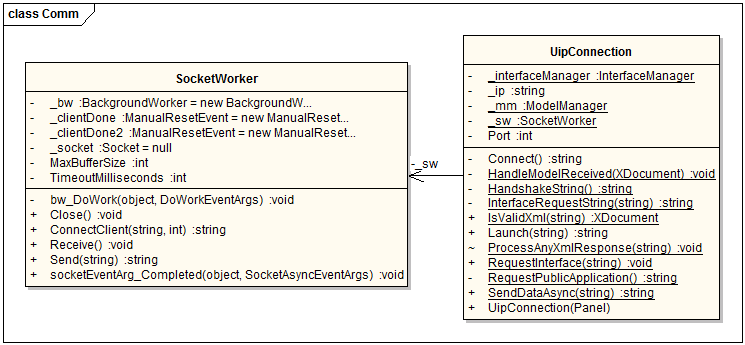
\includegraphics[width=145mm]{pics/3/classComm.png}
\caption{Class diagram of communication classes}
\label{fig:classComm}
\end{figure}

Apart from the mentioned classes that will serve for communicating the XML messages, there there will be another class responsible for acquiring resources (such as images) from the server. For this purpose, the server is awaiting a HTTP connection on another port and the client can open a connection and make a standard HTTP request for the resource. This functionality will be implemented in the \texttt{HttpConnection} class.

\subsection{Parsing XML Into Inner Object Representation}
After the UIP documents will be received by the \texttt{UipConnection} class, they will be passed to instances of \texttt{ModelManager} and \texttt{InterfaceManager} classes.\linebreak \texttt{ModelManager} will be responsible for processing possible new models or model updates and will be discussed later in more detail.

All of the UIP elements need to be represented by objects, so that they are easily manipulated. To create the object representation, \texttt{InterfaceManager} class will process the XML data that describes the UI by recursively traversing the XML tree and creating instances of \texttt{Interface}, \texttt{Container} and \texttt{Element} classes, based on the type of the considered XML node. These instances will represent the UIP elements of the same name - UIP interface, UIP container and UIP element, respectively. This way, every UIP element will be parsed into an inner object representation that will be easy to handle in further work with the objects.

\begin{figure}[ht!]
\centering
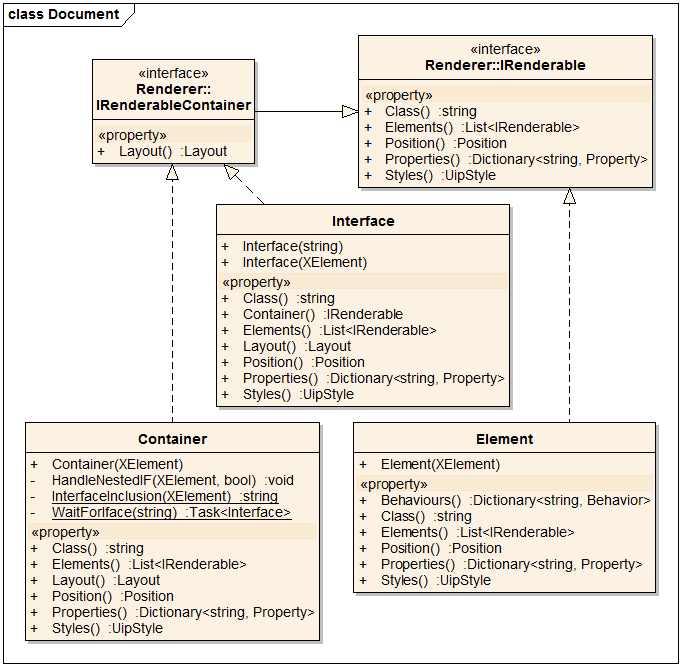
\includegraphics[width=145mm]{pics/3/classDocument2.png}
\caption{Class diagram of the classes representing UIP interface, container and element}
\label{fig:classDocument}
\end{figure}

An important component is the \texttt{IRenderable} interface which is implemented by the \texttt{Interface}, \texttt{Container} and \texttt{Element} classes. This interface represents the functionality all of the classes have in common - most importantly the UIP class (i.e. type of the UI control - see \ref{uipProperty} for example of \texttt{public.input.text} which represents the C\#'s \texttt{TextBox}), UIP properties and contained elements. \texttt{IRenderableContainer} only extends the \texttt{IRenderable} interface by adding a method for obtaining layout. Since layout is a container feature, only \texttt{Interface} and \texttt{Container} classes will implement it.

\subsection{Managing Models and Binding}
To conform the UIP specification, the client must be thin, i.e. it will only store as much data as is needed to render the required interfaces and not execute any code on that data. The data shown to the user can be either constant or come from models, which are designed to be a data storage, as discussed in \ref{subsec:models}. Models will be managed by one instance of \texttt{ModelManager} class.

If an UIP element has a property that refers to a model, \texttt{ModelManager} will be responsible for requesting the model containing this property. Once the model is received, \texttt{ModelManager} will store all its properties and will manage future model updates. Note that the updates can come from the server at any time. \texttt{ModelManager} will also need a reference to \texttt{InterfaceManager} because server's models can contain a request to render an interface. The relationship between classes that are involved in model management is shown in figure \ref{fig:classModel}.

When a UIP property refers to a model, a binding will be created so that when the UIP property is updated, the update is shown in the UI. For that reason there has to be a data binding between the two. We will make use of the data binding API which is built-in to the Windows Phone platform.

\begin{figure}[ht!]
\centering
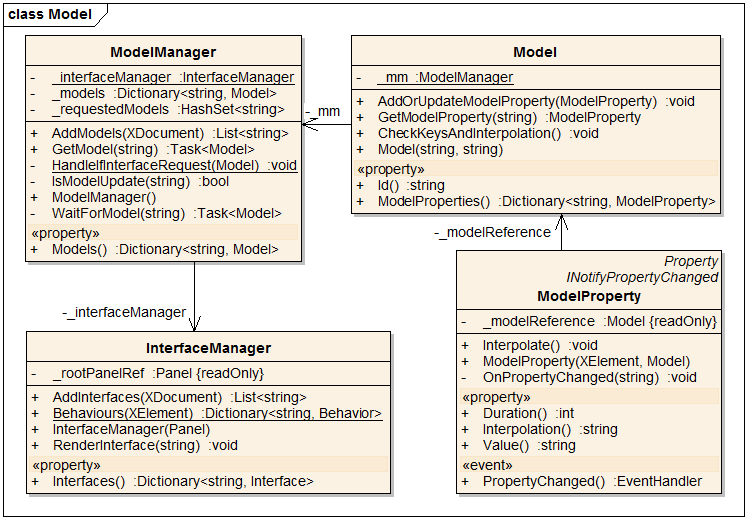
\includegraphics[width=145mm]{pics/3/classModel.png}
\caption{Model and interface management class diagram}
\label{fig:classModel}
\end{figure}

\subsection{Managing Interfaces}
Interface is the root element for all UI controls in UIP documents. An application can contain a large number of interfaces. We therefore need a class to keep the interface information. \texttt{InterfaceManager} will serve as a place for storing information about received and requested interfaces. The most important methods implemented in it will be for adding received interfaces, obtaining an interface and rendering. The process of rendering is described more closely in the next paragraph.

\subsection{Rendering the UI}
The information about UI elements comes from the server in form of XML description. This description is parsed into inner object representation - classes shown in figure \ref{fig:classDocument}. 

After this is done, \texttt{InterfaceManager} will call the \texttt{Render()} method of the \texttt{Renderer} class. This method will traverse the tree of the newly created instances of classes from figure \ref{fig:classDocument} and for each one creates a new class instance which will wrap the platform-native UI controls, as described in the next section.

\begin{figure}[ht!]
\centering
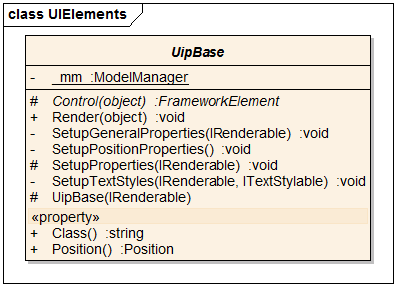
\includegraphics[width=85mm]{pics/3/classUipBase.png}
\caption{UipBase class diagram}
\label{fig:classUipBase}
\end{figure}

\subsection{Representing the Platform-native UI Components}
There is one more step toward the controls that are rendered to the user which involves the transition from the inner object representation to the platform-native components.

The platform-native components will be wrapped into wrapper classes whose names will indicate the component which is wrapped inside (i.e. \texttt{UipPasswordBox} will be the wrapper class of WP8's \texttt{PasswordBox}). There will be an abstract base class, \texttt{UipBase} which will contain everything the wrapper classes have in common: methods for binding to models, and support for styling, element dimensions and positioning.\\
Any particular UI element needs to inherit from the base class in order to support rendering, model updates and other functionality provided by the base class.

\subsection{Events}
The application is designed to support the client-to-server communication in form of events. Events are the only data sent by the client and their intent is to inform server of an user action or request missing data - models.\\\\
Events could be divided into two categories.\\
\begin{description}
  \item[Static] \hfill \\
 Events that are static and are hard-coded within the application. These events are used rarely, typically while going through the procedure of connecting to the server. Currently these are the \texttt{public.connection.connect} and \texttt{public.request. model}, as well as \texttt{public.application}.
  \item[Dynamic] \hfill \\
 Other events are the ones triggered by the user or by the client itself, when it requests a model. These events are dynamic, created at runtime. The event firing - i.e. notifying server of an action taking place, is a relatively simple process which will be handled by two classes. Its working is described in the Implementation chapter.
\end{description}

\begin{figure}[ht!]
\centering
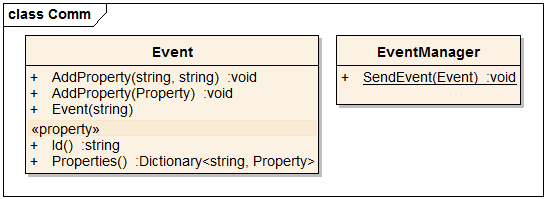
\includegraphics[width=120mm]{pics/3/classEvent.png}
\caption{event class diagram}
\label{fig:classEvent}
\end{figure}

\subsection{Properties}
Properties are the most nested objects in UIP documents. They are used extensively within many classes, including \texttt{Layout}, \texttt{Event} or \texttt{Element}. In all classes they will be stored in dictionaries, identified by their name. The \texttt{ModelProperty} class used in Model will inherit from \texttt{Property} class. 

%They are directly attached to the particular class instance.

\subsection{Layouts}
Windows Phone 8 supports two main types of layouts: absolute and dynamic.
In an absolute layout, child elements are arranged in a layout panel by specifying their exact locations relative to their parent element. Absolute positioning doesn't consider the size of the screen.

In a dynamic layout, the child elements are arranged by specifying how they should be arranged and how they should wrap relative to their parent. With dynamic layout, the user interface appears correctly on various screen resolutions.\\

Both layout types will be supported in our client. Even though absolute layout is not recommended by the accessibility guidelines \cite{wp8guide} it is a basic form of layout and decision has been made to support it.

Layouts are a feature of containers and interfaces which support it through the \texttt{IRenderableContainer} interface. Every container, therefore can place its content into one of the two layouts. As with any property, the positioning will be binding-enabled.

The client will support a container with scrollable content (through \texttt{ScrollViewer}) so that content which does not fit in the screen can be reached by scrolling.

\subsection{Configuration}
Client will have support for basic configuration - i.e. the default IP address and ports on which the socket is tying to connect to the UIP and the HTTP server. Also the constants which are used in the portions of XML throughout the application will be stored in one static class so that they are easy to maintain. 

\subsection{Behaviors}
Behaviors are used to attach event listeners to UI controls. C\# has a built-in support for events through Event and Delegate classes and we will take advantage of it.

Behaviors will be attached to the classes inheriting from \texttt{UipBase} as event handlers. Each handler is for one type of behavior and when the event is fired, the event handler catches it.

\subsection{Interpolation}
The client will support interpolation of UI controls. In the context of UIProtocol, interpolation means animation of UI elements. For example, some action may trigger interpolation which will cause an UI element to move on the screen of the phone. A model update will specify the direction, duration and position where the UI element should move. UIProtocol specifies multiple types of interpolation, our client will only support linear (\texttt{public.number.linear}) and immediate (\texttt{public.immediate}) interpolations.

%\begin{figure}[ht!]
%\centering
%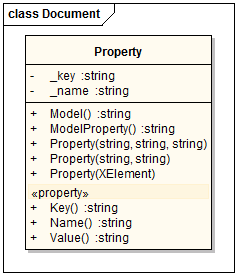
\includegraphics[width=60mm]{pics/3/classProperty.png}
%\caption{properties class diagram}
%\label{fig:classProperty}
%\end{figure}

%positions, interpolace

  \chapter{Implementation}
After providing an analysis of UIProtocol, settling down on the requirements and working out the design of the app, we can now present how the application was being developed, what technologies were used, what problems were encountered and how they were tackled.

\subsubsection{Development Environment}
As previously said, the application was written in the Visual Studio 2013 IDE and using C\#, a programming language developed by Microsoft. The reasons for choosing Visual Studio (VS) are clear: VS is the main development tool for the whole .NET platform, fully supports C\# and Windows Phone development and debugging. VS is therefore the main tool to be used for most .NET development.\\The programming was backed up by running the code directly on a Windows Phone 8 device, namely HTC 8S. We also used ReSharper, a useful plugin for code inspection, maintenance, refactoring and coding assistance.

\subsubsection{Overview of Core Classes}
In this section, we will cover the most important classes of the application, to give a brief idea of how the UIP documents are handled, stored, processed and how the UI is rendered. There are several tables in the following pages, documenting classes for inner UIP Document representation (Table \ref{tab:uipDocClasses}), rendering support (Table \ref{tab:uipRenderClasses}), the communication with the server \ref{tab:uipCommClasses} and the classes for management of interfaces and models \ref{tab:uipManagers}.


\begin{table}[htbp]
  \centering
  \caption{UIP Document Representation Classes}
  \label{tab:uipDocClasses}
 \renewcommand{\arraystretch}{1.2}
    \begin{tabularx}{\textwidth}{p{2.5cm}|X}
    \rowcolor{mygray}
    \textbf{Class Name} & \textbf{Class Description} \\
       Interface & This class represents the UIP interface as a container for more UI elements. This class has its own position, a container and can be embedded into another interface, as specified in Listing \ref{uipInterface}. \\ \hline
       Container & This is the class that stores the information about the particular UI elements. A Container can contain other Containers and instances of Element class.\\ \hline
       Element & Class representing particular UI elements such as button, textfield and more. \\
    \end{tabularx}%
    \label{tab:uipDocClasses2}
\end{table}%

\begin{table}[htbp]
  \centering
  \caption{Classes ensuring the rendering of UI elements}
  \label{tab:uipRenderClasses}
 \renewcommand{\arraystretch}{1.2}
    \begin{tabularx}{\textwidth}{p{3cm}|X}
    \rowcolor{mygray}
    \textbf{Class name} & \textbf{Class description} \\
       Renderer & The main class responsible for rendering the elements stored in the classes of table \ref{tab:uipDocClasses}. Its rendering method walks through the tree structure of UIP Document and invokes rendering of each element. It also does the graceful degradation of unsupported elements. \\ \hline
       IRenderable & An interface which defines methods for acquiring class, style, position and other properties of UIP elements. It is implemented by all classes in table \ref{tab:uipDocClasses}. \\ \hline
       \hspace{0pt}IRenderableContainer & Extension of \texttt{IRenderable} interface. It provides support for layouts and is implemented by instances of Interface and Container. \\
    \end{tabularx}%
\end{table}%

\begin{table}[htbp]
  \centering
  \caption{UIP Server connection classes}
  \label{tab:uipCommClasses}
 \renewcommand{\arraystretch}{1.2}
    \begin{tabularx}{\textwidth}{p{3cm}|X}
    \rowcolor{mygray}
    \textbf{Class name} & \textbf{Class description} \\
      UipConnection & Initiates the connection and is responsible for sending events to the server and processing its responses. Does basic XML validation. \\ \hline
       SocketWorker & Handles the socket communication with UIP server. Sends events and runs a separate thread for receiving server's responses. \\ \hline
       HttpConncetion & Class responsible for acquiring resources via HTTP.
    \end{tabularx}%
\end{table}%

\begin{table}[htbp]
  \centering
  \caption{ModelManager and InterfaceManager classes}
  \label{tab:uipManagers}
 \renewcommand{\arraystretch}{1.2}
    \begin{tabularx}{\textwidth}{p{3cm}|X}
    \rowcolor{mygray}
    \textbf{Class name} & \textbf{Class description} \\
     ModelManager & Keeps and updates all requested and received models. Is implemented as a singleton class. \\ \hline
       \hspace{0pt}InterfaceManager & Stores all received interfaces. Provides getter method and method for rendering an \texttt{Interface}. Is also implemented as a singleton.\\
    \end{tabularx}%
\end{table}%

\subsubsection{Communication With UIP Server}
As mentioned in Table \ref{tab:uipCommClasses}, the communication with server in implemented in \texttt{UipConnection} class which exposes its functionality for sending events to the rest of the application - namely the \texttt{EventManager} class. It also is responsible for processing any XML data received from server that is sent to it from a \texttt{SocketWorker} instance.
\\
\texttt{SocketWorker} is the low-level socket communication class which ultimately sends events to the server, such as interface requests or events informing about user actions. It also runs an instance of \texttt{BackgroundWorker} class which, in an extra thread, awaits data from the server. The reason there is a separate thread for receiving data is that we cannot make any assumptions about when the server will send data to the client. Generally speaking, server can decide to send model updates at any time, not only as a response to a certain user action.\\
The communication was observed from another, already implemented client. todo

\subsubsection{Model Updates and Binding}
Any property of UIP document can, instead of direct value, contain a reference to a model and its property, as described in \ref{subsec:models}. As an example, let us consider a button. The text displayed in the button (its Content) can be either hard-coded into the UIP document or there can be a reference to a model property. If the reference is present, the \texttt{ModelManager} looks into an internally stored dictionary of models and if the model is present, the value of its corresponding property is immediately used. If that is not the case, \texttt{ModelManager} makes a request for the model and once it arrives, its corresponding property's value is used. In both cases, a binding is created so that the future updates of the model property are correctly propagated throughout the application.\\The code which acquires the models and creates binding between model properties and properties of UI elements makes heavy use of asynchronous methods. The async/await operations were introduced with C\# 5.0  and provide a developer with a comfortable way to deal with operations that are potentially blocking. Because requesting and receiving models happens over the internet, it can be considered such. If model request and receive was blocked within a synchronous process, the entire application would be forced to wait. However, by taking advantage of the asynchronous programming, the application continues with other work that doesn't depend on the web resource until the potentially blocking task finishes.

\subsubsection{Interpolations (animations)}
Interpolation allows to move UI controls on the canvas. Because interpolation uses model updates, the prerequisite for it is that the UI control's coordinate which we want to change is bound to a model (i.e. if we want to move a button horizontally, we need to bind the \texttt{x} coordinate of its \texttt{Position} to model). It is implemented through event which is fired by activating the UI control which is to be interpolated. The server responds by a model update which contains "interpolation" and "duration" attributes. The body of the model update contains the value to which the position will be updated. An example of such model update is shown in listing \ref{uipInterpolation}.

\lstinputlisting[label=uipInterpolation,caption=UIP model update specifying interpolation]{sources/uipInterpolation.xml}

Interpolation works through model-wide binding. The \texttt{ModelManager}, when it receives an interpolation model, starts a new \texttt{Task} which periodically updates the given property value (property \texttt{x}, considering our example). Because of the data binding, this update also triggers update of the UI control's position on the canvas, which cause the UI control to move.

Both \texttt{ModelManager} and interface manager classes only need to be instantiated once, so that the application state is stored in one place. Therefore \texttt{ModelManager} and \texttt{InterfaceManager} are singleton classes.

\subsubsection{Binding Converters}
It has been said that any property can be bound to a model. However, properties in UIP document can convey a wide range of information - including color, font size, row and column position in grid and etc. Since the model updates are always received as string, the binding has to be provided with a converter which, considering the given examples, converts the received string to \texttt{SolidColorBrush}, double and integer types, respectively. We implemented several converters which all implement \texttt{IValueconverter} interface.

\subsubsection{Implementing the UI Element Classes}
When deciding how to represent the platform native components which are displayed to the user, we chose to use wrapper classes which will expose the wrapped object's methods and at the same time be able to set up its properties from the UIP document. All supported native components are therefore wrapped into other classes whose names indicate the enclosed UI element (i.e. \texttt{UipButton}) is a wrapper class of standard Button class). All of these wrapper classes inherit from abstract class \texttt{UipBase} which provides a common support for model binding for all inherited components. This way, adding new UI components with binding support is made easy.

The \texttt{ITextStylable} interface is implemented by classes which contain text which can be styled. For example, a \texttt{UipTextBlock} implements this interface in order to be able to set font size, color and more. \texttt{UipContainer}, on the other hand, does not implement it because a container itself does not have anything to style - what about background color?? TODO\\
The figure \ref{fig:UIclasses} shows a class diagram of a few wrapper classes and also \texttt{ITextStylable} being implemented.

\begin{figure}[ht!]
\centering
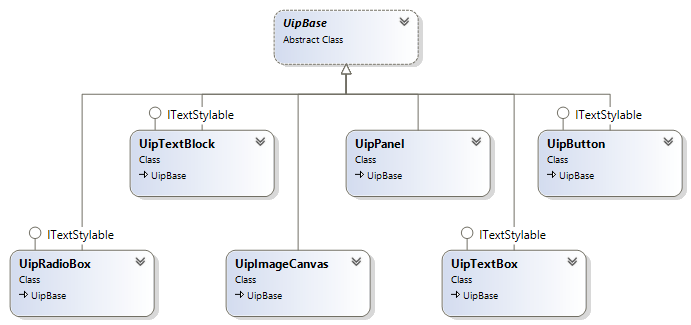
\includegraphics[width=140mm]{pics/UI_classes.png}
\caption{Inheritance tree of several sample UI classes}
\label{fig:UIclasses}
\end{figure}

\subsubsection{Graceful Degradation}
Graceful degradation is a mechanism which replaces unsupported UI elements by supported ones while rendering is being done. This replacement, of course, does not happen without loss. To illustrate this, let us consider the following example:

The server asks the client to render an UIP element of class \texttt{public.input.choice.single} – an UI element known under the WP8 platform as \texttt{ListPicker}. This element, however, may not be supported by the client. If this is the case, the graceful degradation takes place and degrades this to \texttt{public.input.choice} which will be rendered as a group of radiobuttons (assuming this basic UI element is supported).

\subsubsection{Event Communication}
Event management is relatively simple: two classes take care of it.

the code contains a number of string constants that are used to acquire XML elements from the XML documents or to create events that are sent to the server (typically in static methods of the \texttt{UipConnection} or \texttt{Event} classes). To make the maintenance of these constants easy, they are all stored centrally in the \texttt{Consts} class and split into the following categories:

\begin{description}
  \item[UIelements] \hfill \\
  All constants used while parsing the UIP documets into the inner obejct representation. Examples are \texttt{public.scroll} or \texttt{public.input.text}.
    \item[Events] \hfill \\
    Constants used for constructing events such as \texttt{public.request.interface}.
        \item[Styling] \hfill \\
    Constants that have to do with appearance of UI controls or layouts. Example include \texttt{width}, \texttt{font.color} or \texttt{public.grid}.
    \item[General] \hfill \\
  Constants that do not fit into any of the previous categories.
\end{description}

debugging messages

\subsubsection{Configuration}
The client connects to the UIP server and HTTP server on ports that are settled on by the specification ahead of time. The port, default IP address and socket buffer size are all stored in the \texttt{Settings} class where they can be easily modified.

\subsubsection{Problems in Implementation}
We encountered several problems in the development. First issue was related to receiving communication from the server. The difficulty was that the model updates can arrive at any time, not only as a response to a certain user action. The problem was solved by running the receive operation in another thread. This way, the client socket is always ready to receive data.\\

Another issue was related to chained UIP properties. The UIP properties are transitive - consider property \emph{A} whose key refers to property \emph{B}. Property \emph{B} also has a key which points to property \emph{C}. Property \emph{C} contains a constant. The constant has to be propagated back to properties \emph{A} and \emph{B}. Also, when property \emph{C} is updated, the update has to be reflected in properties \emph{A} \emph{B}.
A simple solution would be to create a custom \texttt{DependencyProperty} and then create a binding. However, we were unable to create the chained binding and chose an alternative way instead. Instead of binding, the solution involves creating event listeners. In the example given above, the property \emph{B} would create an event handler that would hook up on changes in \emph{B}'s value. Similarly, property \emph{A} would be listening for updates of \emph{B}.\\

Next, rendering containers of the class \texttt{public.scroll} into grid layout created unnecessary margins of the container.
  \chapter{Testing}
The last task we need to fulfill is to show that the client is able to process UIP documents. In order to do so, we created a testing application.

splneni pozadavku,
testing application
unit testy
novy chapter conclusions / conclusion and future work
slovnicek pojmu a pak \emph{ewew}
prefetching

Testing was primarily done by directly running the developed solution on the provided windows phone device (HTC 8S). Visual Studio offers means for running and debugging the application which allow for fast development. 
We developed a testing app written in UIP XML language which was then run by the developed client. This application covered the testing of switching interfaces, including them, models and their updates, animations and events.

To widen the coverage of testing we also added unit tests which should detect bugs that were not discovered while running the testing application. The unit tests cover the most important classes of the project.

  \chapter{Conclusions and Future Work}
Navigation and mobility are key abilities to a comfortable living. Navigating outdoors is, thanks to global systems such as GPS significantly simplified. Indoor navigation remains a much less developed field. There are research projects that develop solutions for indoor navigation based on various technologies. One of such projects is NUIP from FEE CTU which combines NaviTerier (path planner and directions generator) with UIProtocol.

We analyzed the state of the art in indoor navigation and compared the accessibility features of the most common smartphone platforms. The reader was also introduced to UIProtocol, its architecture and how it functions.

The goal of the thesis was to implement an UIProtocol client supporting the basic features every UIP client needs to support. The platform of development was chosen to be Windows Phone 8. The client was expected to be able to be used within the NUIP project and consequently, we researched ways of making it more accessible to people with disabilities. We found, however, that the Windows Phone 8 platform is not suitable for visually impaired.

\section{Current Features}
Within the bachelor thesis we successfully implemented a basic UIProtocol client which implements:

\begin{description}
  \item[Basic UI controls] \hfill \\
  
  \item[Binding and model-wide binding] \hfill \\
  \item[Graceful degradation for unsupported elements] \hfill \\
  \item[Support for UI generator API] \hfill \\
  todo
  \item[Support for interpolated model updates (animations)] \hfill \\
  \item[Support for absolute and grid layouts] \hfill \\\\
  \item[Support for styling] \hfill \\\\
\end{description}

The features we implemented completely cover the functional requirements we have set in the Design chapter.

The non-functional requirements were also met. The UI loading times are below 0.5 s in all interfaces of the testing application. The execution profiling has shown increased CPU usage in some situations, but when idle, the consumption of phone's resources is normal.

\section{Future Work}
Implementing the full feature set of an UIProtocol client was not possible in the scope of this work. Therefore there is a number of features by which the client could be extended. In particular the extensions may include:

\begin{description}
  \item[StackPanel layout panel] \hfill \\
  The StackPanel is a simple layout panel that arranges its child elements into a single line that can be oriented horizontally or vertically. Currently, the app supports Grid and Canvas panels to which UI controls can be added. StackPanel should be implemented to widen the choice of layout panels. 
  \item[More UI controls] \hfill \\
  The client comes with a small set of implemented UI controls. New UI controls can be implemented, such as an audio element.
  \item[Wider support for styling] \hfill \\
  The app could implement more font styles, such as font family, font type (e.g. italic, bold).
  \item[Performance optimization] \hfill \\
  The performance of the current client is satisfactory, it could, however be improved by techniques such as interface pre-fetching.
  \item[Error handling] \hfill \\
  The client ignores errors received from the server, for example if a requested interface is not found at the server.
  \item[Support for different screen orientations] \hfill \\
When a user rotates the phone, the UI remains the same. this is not so important for the nuip project but an UIProtocol client should have this feature implemenred
refreshing only parts of UI that need to be refreshed.
\item[Screen reader friendliness] \hfill \\
Currently, the implementation redraws the whole UI. This approach was chosen for its simplicity. This approach, however, is not discouraged by the accessibility guidelines for WP8. todo toto bych mozna stihl predelat.
\end{description}




  
  \startAppendices
    \chapter{Speech Accessibility Features}
The following two tables describe the speech commands which can be used in WP8 and iPhone, respectively.
% Table generated by Excel2LaTeX from sheet 'List1'
\begin{table}[htbp]
  \centering
  \caption{Windows Phone 8 Speech Commands}\label{tab:w8sc}
  \renewcommand{\arraystretch}{1.2}
    \begin{tabularx}{\textwidth}{p{3cm}|X}
    \rowcolor{mygray}
    \textbf{Operation}  & \textbf{Say this} \\
    Call someone from your contact list & "Call contact name" 
           (where contact name is the name of someone in your contact list) 
           If the person has only one phone number in your contact card, the call will start. If he or she has multiple phone numbers, you'll see an option to choose one. \\ \hline
    Call any phone number & "Call phone number" (where phone number is any phone number, whether it belongs to a contact or not)\\ \hline
     Redial the last number & "Redial" \\ \hline
    Send a text message & "Text contact name" (where contact name is the name of someone in your contact list). This will start a text message to that person. Then you can dictate and send the message—hands-free. \\ \hline
    Call your voicemail & "Call voicemail" \\ \hline
    Open an application & "Open application" or "Start application" (where application is the name of any application on your phone, such as "Calendar," "Maps," or "Music") \\ \hline
    Search the web & "Find search term" or "Search for search term" (where search term is what you're looking for). If you say "Find local pizza," for example, Bing will bring up a map of nearby pizza places. \\ \end{tabularx}
\end{table}%

% Table generated by Excel2LaTeX from sheet 'List1'
\begin{table}[htbp]
  \centering
  \caption{Android speech commands (from \cite{googleNow})}
  \label{tab:asc}
 \renewcommand{\arraystretch}{1.2}
    \begin{tabularx}{\textwidth}{p{3cm}|X|X}
    \rowcolor{mygray}
    \textbf{Say} & \textbf{Followed by} & \textbf{Examples} \\
    "Open" & App name & "Open Gmail" \\ \hline
   "Show me my schedule for the weekend." &       & Say "What does my day look like tomorrow?" to see tomorrow's agenda. \\ \hline
    "Create a calendar event" & "Event description" \& "day/date" \& "time" & "Create a calendar event: Dinner in San Francisco, Saturday at 7:00PM" \\ \hline
    "Listen to TV" & Displays TV cards relevant to the TV show that's currently being broadcast & While a TV show is being broadcast, say "Listen to TV" \\ \hline
    "Map of" & Address, name, business name, type of business, or other location & "Map of Golden Gate Park, San Francisco." \\ \hline
    "Directions to" or & Address, name, business name, type of business, or other destination & "Directions to 1299 Colusa Avenue, Berkeley, California" or \\ \hline
    "Navigate to" &       & "Navigate to Union Square, San Francisco." \\ \hline
    "Post to Google+" & What you want posted to Google+ & "Post to Google+ I'm going out of town." \\ \hline
    "What's this song?" &       & When you hear a song, ask "What's this song?" \\ \hline
    "Remind me to" & What you want to be reminded about, and when or where & "Remind me to call John at 6PM." \\ \hline
    "Go to" & Search string or URL & "Go to Google.com" \\ \hline
    "Send email" & "To" \& contact name, "Subject" \& subject text, "Message" \& message text (speak punctuation)  & "Send email to Hugh Briss, subject, new shoes, message, I can’t wait to show you my new shoes, period." \\ \hline
    "Note to self" & Message text & "Note to self: remember the milk" \\ \hline
    "Set alarm" & "Time" or "for" \& time, such as "10:45 a.m." or "20 minutes from now," "Label" \& name of alarm & "Set alarm for 7:45 p.m., label, switch the laundry" \\ \hline
    "Call" & The name of one of your contacts & "Call George Smith" \\ \end{tabularx}%
\end{table}%

  \stopAppendices
\stopBodyMatter

\startBackMatter
  \PrintBibliography
  %\PrintIndex % define index entry in the text by: \index{word}
\stopBackMatter

\end{document}

\endinput
%%
%% End of file